\documentclass[../DoAn.tex]{subfiles}
\begin{document}

Trong chương 5 này, em sẽ trình bày tất cả những nội dung đóng góp mà em cảm thấy tâm đắc nhất trong suốt quá trình làm đồ án.

\section{Sử dụng realtime - Socket.IO}
\subsection{Đặt vấn đề}

Trong một hệ thống điều khiển từ xa, điều quan trọng nhất chính là trải nghiệm người dùng khi sử dụng, thực hiện các thao tác giữa các thiết bị với nhau. Một chiếc xe nhận tín hiệu từ ứng dụng chậm sẽ gây cảm giác rất khó chịu, ức chế đến người dùng. Một trong những nguyên nhân gây nên việc xử lý gửi/nhận thông tin chậm đó là cách server xử lý thông tin và thiết bị tiếp nhận thông tin từ server.

Vì vậy, server nảy sinh ra 2 vấn đề:
\begin{itemize}
    \item Server mất thời gian nhận thông tin từ ứng dụng, xử lý thông tin.
    \item Thiết bị Arduino nhận thông tin từ server và tiếp tục xử lý để thực hiện hành vi.
\end{itemize}

\subsection{Giải pháp}
Với các vấn đề nêu trên, em dùng một công cụ giúp thực hiện những ứng dụng realtime đó là Socket.IO. Ở đây, Socket.IO được sử dụng kết hợp với NodeJS. Ở phía server sẽ là nơi đặt Socket.IO để lắng nghe và truyền dữ liệu. Ở phía client cũng cần sử dụng Socket.IO để lắng nghe dữ liệu và truyền dữ liệu về server. Với cơ chế hoạt động thời gian thực của Socket.IO sẽ giảm được độ trễ rất nhiều.

\begin{figure}[H]
    \centering
    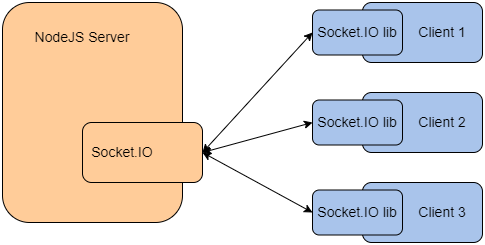
\includegraphics[scale = 0.75]{Hinhve/socketio.png}
    \caption{Sơ đồ sử dụng socket.IO kết nối giữa Server và Client}
    \label{fig:Fig0}
\end{figure}

Hình \ref{fig:Fig0} mô tả cách sử dụng Socket.IO trong hệ thống có Server và Client. Trong hệ thống của em, các Client là ứng dụng điện thoại và thiết bị Arduino sẽ sử dụng thư viện có Socket.IO để kết nối với một Server NodeJS giúp trao đổi thông tin một cách nhanh chóng, tức thời.

\section{Ứng dụng đa nền tảng - Flutter}
\subsection{Đặt vấn đề}

Về trải nghiệm người dùng khi sử dụng hệ thống, ngoài tốc độ xử lý nhanh giữa Server và Client, bên cạnh đó các thao tác trên ứng dụng điện thoại cũng là vấn đề đáng được quan tâm cho những người lập trình Mobile Application. Hãy thử hình dung một ứng dụng có những đặc điểm sau đây:

\begin{itemize}
    \item Các tiêu đề, nút ấn, biểu tượng không đồng nhất về màu sắc, kích thước, vị trí.
    \item Khi lấy dữ liệu về hoặc truyền dữ liệu lên không có loading để người dùng thoải mái thực hiện các thao tác khác.
    \item Di chuyển giữa các màn hình bị giật, không mượt mà.
\end{itemize}

Vậy chúng ta sẽ xử lý những vấn đề này để cho người dùng lúc sử dụng sẽ không cảm thấy khó chịu.

\subsection{Giải pháp}

\begin{figure}[H]
    \centering
    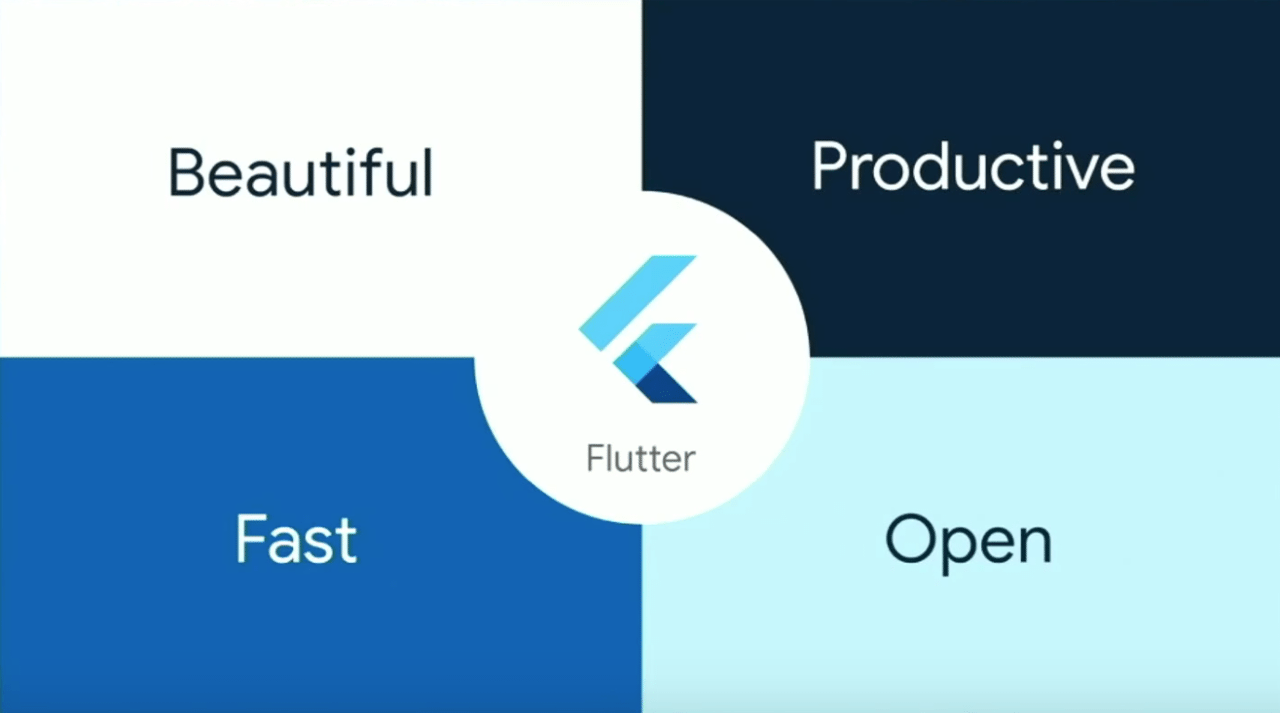
\includegraphics[scale = 0.3]{Hinhve/flutter.png}
    \caption{Framework Flutter sử dụng trong ứng dụng}
    \label{fig:Fig1}
\end{figure}

Với những vấn đề nêu trên, em đã tìm hiểu và lựa chọn Flutter là framework phát triển ứng dụng cho ĐATN của em. Flutter có một kiến trúc lớp cho phép các nhà phát triển điều khiển mọi pixel trên màn hình, nó giúp đồng bộ hoá các thành phần như tiêu đề, nút nhấn, hình ảnh và nhiều những thành phần cần dùng khác. Flutter sử dụng ngôn ngữ lập trình chính là Dart, Dart được phát triển bởi Google và dành cho các ứng dụng di động, máy tính, backend và kể cả ứng dụng web. Dart giúp tối ưu hoá phía client để người dùng thực hiện nhanh các ứng dụng trên nhiều nền tảng. Ngôn ngữ này biên dịch nhanh, dự đoán tốt. Điều này làm cho Flutter cực kỳ nhanh và có thể tuỳ chỉnh hầu như tất cả mọi thứ trong ứng dụng.

Sau khi sử dụng Flutter, ứng dụng có thể chạy tốt trên 3 nền tảng là Android, iOS và Web, ngoài ra ứng dụng đem lại trải nghiệm mượt mà, động bộ.

\section{Sử dụng cảm biến khoảng cách - HC-SR04}
\subsection{Đặt vấn đề}

Trong quá trình xe Arduino di chuyển, người dùng sẽ không phát hiện kịp thời nếu như có một vật cản bất ngờ xuất hiện trước xe. Ở đây chúng ta gặp 2 vấn đề:

\begin{itemize}
    \item Thứ nhất, làm sao để xe Arduino phát hiện được vật cản trước mặt và thông báo về ứng dụng.
    \item Thứ hai, xe Arduino sẽ xử lý thế nào nếu gặp vật cản.
\end{itemize}

\subsection{Giải pháp}

Về vấn đề thứ nhất, em đã sử dụng HC-SR04, thiết bị này là cảm biến siêu âm được sử dụng để xác định khoảng cách của đối tượng phía trước. Ở đây, thiết bị này sẽ phản hồi liên tục khoảng cách tới vật cản trước mặt về Server, phía ứng dụng sẽ hiển thị khoảng cách liên tục, nếu dưới 20cm sẽ thông báo tới người dùng. Nếu như gặp vật cản, xe Arduino sẽ nháy đèn đỏ và dừng lại.

\end{document}